\chapter{Design}

In Kapitel \ref{chap:2} wurde die PSI-Theorie detailliert beschrieben. Sie erklärt verschiedene Funktionszustände eines Menschen, und liefert damit eine fundierte Grundlage für die Entwicklung eines KI-basierten Chatbots, der im Coaching Bereich einsetzbar sein soll. Im Folgenden wird ein Modell konzeptionell beschreiben, dass diese Kriterien erfüllt und somit als Werkzeug für Coachings mit traumasensibler Ausrichtung dienen soll. Es wird eine PSI-basierte Dialogsteuerungslogik für ein traumasensibles Coaching-System entwickelt und evaluiert. Ziel des Modells ist, es dem hohen Bedarf an Coaches und Therapeuten entgegenzuwirken, indem zu persönlichen Denk- und Entscheidungsmustern weitere Optionen und Handlungsmöglichkeiten offenbart werden. Menschen agieren aufgrund ihrer Prägung, Erziehung, Sozialisierung oder Traumatisierung oft nach ihnen bekannten Strategien. Dadurch besteht das Problem, oft in persönlichen Verhaltensmustern festzuhängen \citep{re1989compulsion}. Das KI-Modell soll an dieser Stelle ansetzen und eine Unterstützung gewährleisten. Der Fokus des Modells liegt auf leichten bis moderaten Belastungen. Für Klienten, die sich in einem solchen Zustand befinden, soll es als ein Tool zur Selbstregulierung und -entwicklung dienen. Für Personen mit schweren Belastungszuständen ist das Modell hingegen nicht geeignet. Es wird davon ausgegangen, dass in solchen Fällen eine professionelle Hilfe, beispielsweise einee therapeutische oder klinische Behandlung, herangezogen werden sollte.

Fokus des entwickelten Modells ist es, selbstregulatorische Prozesse zu unterstützen. Damit sollen Erregungszustände und intensive Emotionen verarbeitet und Traumaheilung gefördert werden. Die Grundidee eines reflektierenden KI-Systems ist, dass es nicht nur auf Aussagen reagiert, sondern zusätzlich individuelle Muster des Nutzers erkennen und im Gesprächsverlauf aufgreifen kann. Es soll keine klinische Diagnose oder Bewertung der Strategien vorgenommen werden, sondern durch ein sichtbar machen die persönliche Selbstreflexion gefördert werden. Spiegelung individueller Muster meint, wiederkehrende Verhaltensmuster zu erkennen und diese aktiv infrage zu stellen. Das KI-System soll somit zur Reflexion und potenziellen Veränderung beitragen, indem dem Nutzer zusätzliche Perspektiven aufgezeigt werden \citep{Xiao2025Humanizing}. Persönlichkeitsentwicklung lässt sich durch das Zusammenspiel der vier psychischen Systeme erklären. Selbstregulationsfähigkeiten entwickeln sich insbesondere in Beziehungen und gegenseitiges Verstehen gilt als wichtige Voraussetzung für Entwicklung \citep{kuhl2005neue,kuhl2014psi}. Für die Übertragung auf die Mensch-Maschine-Interaktion bedeutet das, der Nutzer soll sich verstanden fühlen, individuelle Perspektiven aufgegriffen, sowie Erfahrungen und Bedürfnisse berücksichtigt werden. Interaktion sollen nicht ausschließlich auf eine schnelle Problemlösung ausgerichtet sein, sondern stattdessen ein Raum für Reflexion und Selbstwahrnehmung geschaffen werden.

\section{Integriertes Framework}
Die strukturelle Ausgangsbasis des PSI-Coaching Frameworks bilden das MIND-SAFE und DTx-Komponentenmodell, die in Kapitel~\ref{modell} beschrieben wurden. Die PSI-Theorie liefert zusätzlich eine spezifische Steuerungs- und Adaptionslogik, durch die die bestehenden Komponenten erweitert werden. Im Folgenden wird das Modell ausführlich erklärt. \\
Grundlegend besteht das Modell aus 7 aufeinanderfolgenden Ebenen. Die erste Ebene spiegelt die Nutzereingabe wider. Hier formuliert der Nutzer des Systems sein Anliegen. Im zweiten Schritt folgt eine Sicherheitsprüfung basierend auf der Logik des MIND-SAFE Frameworks \citep{boit2025prompt}. Das bedeutet konkret, dass das System prüft, ob möglicherweise eine akute Gefährdung, wie beispielsweise Suizidalität vorliegt. In diesem Fall würde eine Eskalation erkannt werden und der Nutzer an eine professionelle Hilfestelle weitergeleitet werden. Ist das Ergebnis des Sicherheitschecks nicht kritisch, kommt die nächste Ebene, in der eine PSI-Zustandsanalyse durchgeführt wird. Dieser Schritt ist ein spezifisch für das Modell entwickelte Bestandteil. Dabei werden die Eingaben und Kontextinformationen analysiert. Die Bestimmung des funktionalen PSI-Zustandes erfolgt auf Basis mehrerer Kriterien. Diese orientieren sich an den 7 Systemebenen der Entwicklungsorientierten Osnabrücker Systemdiagnostik \citep{kuhl2004systemdiagnostik}. Das Ergebnis stellt dann eine PSI-Zustandshypothese dar (z.B. OES-dominant). Darauf folgt dann die PSI-Entscheidungsebene, die PSI-basierte Ziele definiert und untersucht, welches für die gegebene Situation passend ist. Auf dieser Grundlage wird geprüft, wie ein möglicher Wechsel der Systeme durch Steuerungsmechanismen möglich ist. In der nächsten Ebene wird dann eine passende Intervention ausgewählt. Dem liegt die Frage zugrunde, welche PSI-Funktion gefördert werden soll. Die Auswahl erfolgt nach dem DTx-Modell. Interventionsziel und -typ ergeben sich aus der Therapie- und Interventionseinheit, der Entscheidungslogik, narrativen Ebene, Unterstützungsfunktion und der therapeutischen Gesprächsinstanz. Abschließend erfolgt die Generierung der Antwort an den Nutzer. Im Gesamten basiert dieser Schritt auf dem Nutzerzustand, PSI-Ziel, der gewählten Intervention, Coaching-Prinzipien und Sicherheitsvorgaben. Am Ende und damit in der letzten Ebene erfolgt ein Update des Zustandes und Feedback. Durch die Nutzerreaktion und neuer Kontextinformationen wird der PSI-Zustand aktualisiert und damit eine Grundlage für die nächste Interaktion geschaffen.
Allildung \ref{fig:psi-chatbot-ablauf} stellt den Ablauf des entwickelten PSI-basierten Chatbots dar. Die einzellnen Schritte und Ebenen werden im Folgenden detailliert beschrieben.

\begin{figure}[htbp]
\centering
\resizebox{0.95\textwidth}{!}{%
\begin{tikzpicture}[
    node distance=8mm and 15mm,
    >=Stealth,
    process/.style={
        rectangle, rounded corners=2pt,
        draw=black, align=center,
        text width=5.0cm, minimum height=9mm,
        inner sep=5pt
    },
    decision/.style={
        diamond, aspect=2.1, draw=black,
        align=center, text width=3.4cm,
        inner sep=2pt
    },
    terminal/.style={
        rectangle, rounded corners=5pt,
        draw=black, align=center,
        text width=4.2cm, minimum height=9mm,
        inner sep=5pt
    },
    intervention/.style={
        rectangle, rounded corners=2pt,
        draw=black, align=center,
        text width=4.2cm, minimum height=9mm,
        inner sep=5pt
    },
    line/.style={->, thick}
]

% Hauptablauf
\node[terminal] (start)
    {Nutzereingabe $U_t$};

\node[process, below=of start] (safety)
    {Sicherheitsprüfung $S_t$};

\node[decision, below=of safety] (risk)
    {Schwere Belastung oder\\
     relevantes Sicherheitssignal?};

\node[terminal, right=of risk] (stop)
    {Interaktion beenden\\
     und an professionelle\\
     Unterstützung verweisen};

\node[process, below=of risk] (context)
    {Kontextanalyse $K_t$ und\\
     PSI-Zustandsanalyse $Z_t$};

\node[process, below=of context] (goal)
    {PSI-Zielermittlung $G_t$};

% Interventionsentscheidungen
\node[decision, below=of goal] (checkI2)
    {$\tau_{m1}>30\%$ und $A^+<0$?};

\node[intervention, left=of checkI2] (onlyI1I2)
    {Interventionen\\
     $I_1=1,\ I_2=1,\ I_3=0$};

\node[decision, below=of checkI2] (checkI3)
    {$\tau_{m2}>30\%$ und $A^->0$?};

\node[intervention, right=of checkI3] (onlyI1I3)
    {Interventionen\\
     $I_1=1,\ I_2=0,\ I_3=1$};

\node[intervention, below=of checkI3] (onlyI1)
    {Nur übergeordnete Intervention\\
     $I_1=1,\ I_2=0,\ I_3=0$};

% Zusammenführung der drei Fälle
\node[process, below=20mm of onlyI1] (generation)
    {Gesprächsgenerierung $R_t$};

\node[process, below=of generation] (update)
    {Antwort ausgeben und Nutzerzustand aktualisieren};

% Verbindungen: Hauptablauf
\draw[line] (start) -- (safety);
\draw[line] (safety) -- (risk);

\draw[line] (risk.east) -- node[above, align=center]
    {Ja} (stop.west);

\draw[line] (risk.south) -- node[right]
    {Nein} (context.north);

\draw[line] (context) -- (goal);
\draw[line] (goal) -- (checkI2);

% Verbindungen: Interventionsauswahl
\draw[line] (checkI2.west) -- node[above]
    {Ja} (onlyI1I2.east);

\draw[line] (checkI2.south) -- node[right]
    {Nein} (checkI3.north);

\draw[line] (checkI3.east) -- node[above]
    {Ja} (onlyI1I3.west);

\draw[line] (checkI3.south) -- node[right]
    {Nein} (onlyI1.north);

% Zusammenführung der Interventionspfade
\draw[line] (onlyI1I2.south) |- (generation.west);
\draw[line] (onlyI1I3.south) |- (generation.east);
\draw[line] (onlyI1.south) -- (generation.north);

% Gesprächsverarbeitung und Rückkopplung
\draw[line] (generation) -- (update);

\end{tikzpicture}%
}
\caption{Entscheidungs- und Verarbeitungsablauf des PSI-basierten
Chatbot-Modells im traumasensiblen Coaching.}
\label{fig:psi-chatbot-ablauf}
\end{figure}


\section{Versuchsaufbau}
Grundlage des Versuchsaufbaus stellt ein experimentelles Design \citep{rubin2008comment} geppart mit einem Within-Scenario-Vergleich dar. Der Begriff und die Analyse wurde von \cite{eisenhardt2009building} geprägt und dient der inhaltlichen und kontextbezogenenen Analyse eines Szenarios beziehungsweise Fallbeispiels. Der aus dem Framework abgeleitete PSI-basierte Chatbot soll mittels Szenarien getestet werden. Dafür soll ein kontrollierter Vergleich zweier Chatbot-Varianten durchgeführt werden. Als Kontrollgruppe wird ein konventioneller LLM-Chatbot herangezogen und als Experimentalgruppe der PSI-basierte Chatbot. Beide Modelle erhalten den identischen Basis-Prompt, während der PSI-Chatbot zusätzlich die entwickelte PSI-Steuerungslogik erhält.

Der Versuchsaufbau dient dazu zu überprüfen, wie das PSI-basierte Chatbot-Modell im Vergleich zu einem konventionellen Chatbot funktioniert. Es werden die zwei experimentelle Bedingungen $B$ untersucht:
\begin{itemize}
    \item $B_{\text{Kontrolle}}(B_K)$: konventioneller Chatbot ohne PSI-basierte Dialogsteuerung
    \[U_t 
\rightarrow S_t
\rightarrow K_t
\rightarrow R_t\]
    \item $B_{\text{PSI}}(B_P)$: Chatbot auf Grundlage des entwickelten PSI-Modells
    \[U_t
\rightarrow S_t
\rightarrow K_t
\rightarrow Z_t
\rightarrow G_t
\rightarrow I_t
\rightarrow R_t
\]
\end{itemize}

mit:
\[
\begin{aligned}
U_t &:= \text{Nutzereingabe zum Zeitpunkt } t,\\
S_t &:= \text{Sicherheitsprüfung zum Zeitpunkt } t,\\
K_t &:= \text{Kontextanalyse zum Zeitpunkt } t,\\
Z_t &:= \text{PSI-Zustandsanalyse zum Zeitpunkt } t,\\
G_t &:= \text{Bestimmung des Unterstützungsziels zum Zeitpunkt } t,\\
I_t &:= \text{Auswahl der Intervention zum Zeitpunkt } t,\\
R_t &:= \text{generierte Chatbot-Antwort zum Zeitpunkt } t.
\end{aligned}
\]

Die beide Modelle bekommen dieselben Grundbedingungen. Für den Versuch wird das Modell gemini-3.8-flash herangezogen. Der Prompt beinhaltet für beide Bedingungen eine identisch definierte Sicherheitslogik, traumasensible Kommunikationsregeln, Coaching-Rolle und gleiche Nutzerinputs. Die beiden Modelle unterscheiden sich nur noch hinsichtlich der PSI-basierten Entscheidungslogik, bestehend aus PSI-Zustand, angestrebtem PSI-Ziel und Interventionsauswahl als Steuerungsmechanismus. Diese mehrstufige Entscheidungslogik dient somit als Kontrollvariable. 
Der Versuchsaufbau besteht aus 2 Szenarien, entsprechend der beiden Modulationsannahmen. 

\begin{enumerate}
    \item \textbf{Szenario 1 (Basisszenario $\mathcal{X}_{M1}$):} Bezug zur ersten Modulationsannahme (M1 - Willensbahnung)
    \item \textbf{Szenario 2 (Basisszenario $\mathcal{X}_{M2}$):} Bezug zur zweiten Modulationsannahme (M2 - Selbstentwicklung)
\end{enumerate}

Um die Funktionsweise der Chatbot-Modell ausreichend testen zu können, werden die Szenarien 100 mal durchlaufen und anschließend die Ergebnisse der beiden Bedingungen $B_{\text{Kontrolle}}$ und $B_{\text{PSI}}$ gegenübergestellt. 
Die formale Stichprobenarchitektur ist als ein $2 \times 2 \times 100$-faktorielles Design definiert (2 Modulationsannahmen $\times$ 2 experimentelle Bedingungen $\times$ 100 iterative Durchläufe). Daraus ergibt sich die Gesamtmenge der zu evaluierenden Datenzeilen ($N_{Total}$) wie folgt:

\begin{equation}
    N_{Total} = \left( 1\text{ Szenario}_{\mathcal{X}_{M1}} \times 100\text{ Iterationen} \times 2\text{ Bedingungen } [B_{PSI}, B_{K}] \right) 
\end{equation}
\begin{equation*}
    + \left( 1\text{ Szenario}_{\mathcal{X}_{M2}} \times 100\text{ Iterationen} \times 2\text{ Bedingungen } [B_{PSI}, B_{K}] \right) = 400\text{ Datenzeilen}
\end{equation*}


\subsection{Technische Umsetzung}

Um den theoretisch hergeleiteten Versuch über insgesamt $N = 400$ Simulationsläufe hinweg systematisch zu vergleichen, wurde eine programmgesteuerte Prüfumgebung in der Programmiersprache Python implementiert. 

Auf diese Weise wird sicher gestellt, dass jeder einzelne Simulationsdurchlauf isoliert betrachtet wird, um kontextuelle Verzerrungen innerhalb des Sprachmodells auszuschließen. Zu diesem Zweck wird bei jeder Iteration ein frischer API-Aufruf generiert, welcher das System-Prompt der jeweiligen experimentellen Bedingung ($B_{PSI}$ bzw. $B_K$) mit dem identischen, statischen Nutzer-Eingabetext ($U_t$) des entsprechenden Basisszenarios kombiniert.

\subsubsection{Ausgewähltes Sprachmodell: Gemini}

Für die Durchfühung des Experiments wird das Sprachmodell Gemini-3.8-flash von Google verwendet. Das Modells liefert eine hohe Performanz bei der Verarbeitung detaillierter System-Anweisungen und zeigt hohe Effizienz. Über das offizielle Google GenAI SDK lässt sich das Modell direkt in das Python-Skript einbinden.

Um eine hinreichende sprachliche und stochastische Varianz in den Ausgaben des Modells zu gewährleisten, ohne die strukturelle Einhaltung der deterministischen Verarbeitungs-Pipeline zu gefährden, wird der Modell-Parameter Temperatur gesetzt:
\begin{equation}
    \text{Temperature} = 0{,}7
\end{equation}

\subsubsection{Erstellung des Ergebnis-Datensatzes}

Da die Rohausgabe eines Large Language Models standardmäßig als unstrukturierter Freitext vorliegt, wurde ein zweistufiges Sicherungsverfahren implementiert, um die qualitativen Coaching-Dialoge von den quantitativen systemdiagnostischen Metriken sauber zu trennen. Der System-Prompt steuert die internen Berechnungen und Klassifikationen nach einem strikten XML-Schema. 
Das in Python implementierte Skript greift nach jedem erfolgreichen API-Call auf die Rohantwort des Modells zu und extrahiert diese Zeile. Im Ergebnis entsteht entsteht ein relationaler Datensatz mit 400 Datenzeilen.


\subsection{Sicherheitsprüfung}

Die Sicherheitsprüfung bildet nach der Nutzereingabe die zweite Ebene des Systems und orientiert sich an den NICE-Leitlinien \citep{kendrick2012common}. Sie stellt somit ein wichtiges Designprinzip des entwickleten Frameworks dar, welches für beide geprüften Bedingungen herangezogen wird. Ziel dieser Ebene ist es, anhand der Nutzereingabe eine strukturierte Bewertung der psychischen Belastung vorzunehmen und potenzielle Sicherheitssignale zu erkennen. Dabei wird zwischen milden, moderaten und schweren Belastungszuständen unterschieden.
Bei einer milden oder moderaten Belastung wird die Interaktion mit der anschließenden PSI-Zustandsanalyse fortgesetzt. Wird hingegen eine schwere Belastung beziehungsweise ein relevantes Sicherheitssignal erkannt, wird die weitere Verarbeitung durch das System beendet und der Nutzer an professionelle Unterstützung verwiesen. Die Sicherheitsprüfung dient somit insbesondere dazu, Situationen zu erkennen, in denen eine weitere Interaktion mit dem System nicht angemessen ist.

Für die strukturierte Einordnung werden mehrere Dimensionen berücksichtigt:

\begin{itemize}
    \item \textbf{Symptomatik:} gering / moderat / hoch
    \item \textbf{Dauer der Symptomatik:} kurz / länger andauernd
    \item \textbf{Alltagsbeeinträchtigung:} gering / deutlich / stark
\end{itemize}

Diese Kriterien werden dem Modell in strukturierter Form vorgegeben. Das LLM extrahiert auf Grundlage der Nutzereingabe die relevanten Merkmale und gibt diese als strukturierte Daten aus.
Das LLM stellt dabei keine medizinische Diagnose und klassifiziert keinen klinischen Zustand im diagnostischen Sinne. Stattdessen liefert es eine strukturierte Einschätzung der zuvor definierten Merkmale. Diese Einschätzung dient als Grundlage für die nachgelagerte regelbasierte Sicherheitslogik. Die eigentliche Entscheidung über die weitere Systemaktion erfolgt somit nicht ausschließlich durch das LLM, sondern durch explizit definierte Entscheidungsregeln. Dadurch soll insbesondere sichergestellt werden, dass sicherheitskritische Zustände nachvollziehbar und konsistent behandelt werden. Sind Symptomatik, Dauer und Alltagsbeeinträchtigung jeweils niedrig beziehungsweise kurz ausgeprägt, wird die Interaktion fortgesetzt.
Für einen schweren Belastungszustand greifen hingegen strengere Entscheidungsregeln. Werden beispielsweise eine hohe Symptomlast und eine starke Alltagsbeeinträchtigung festgestellt, wird der Zustand als schwer eingestuft und die Interaktion beendet. In diesem Fall erfolgt eine Weiterleitung an professionelle Unterstützung.
Die Sicherheitsprüfung fungiert damit als vorgeschaltete Kontrollinstanz. Während das LLM die aus der Nutzereingabe ableitbaren Merkmale strukturiert erfasst, bestimmen die explizit definierten Entscheidungsregeln die daraus resultierende Systemaktion. Die Trennung zwischen sprachmodellbasierter Merkmalsextraktion und regelbasierter Sicherheitsentscheidung erhöht dabei die Nachvollziehbarkeit und reduziert die Abhängigkeit von einer ausschließlich generativen Entscheidung des LLM.
Algorithmus \ref{alg:sicherheitspruefung_gesamt} stellt die regelbasierte Sicherheitsprüfung dar.

\begin{algorithm}[htbp]
\caption{Regelbasierte Logik der Sicherheitsprüfung ($S_t$)}
\label{alg:sicherheitspruefung_gesamt}
\begin{algorithmic}[1]
    \Statex \textbf{1. Strukturierte Merkmalsextraktion (Output des LLM):}
    \State \texttt{symptom\_burden} $\gets$ \texttt{moderate} \Comment{[low / moderate / high]}
    \State \texttt{duration} $\gets$ \texttt{long} \Comment{[short / long]}
    \State \texttt{functional\_impairment} $\gets$ \texttt{high} \Comment{[low / high]}
    \State \texttt{safety\_signal} $\gets$ \texttt{false} \Comment{[true / false]}
    \State \texttt{confidence} $\gets$ 0.86 \Comment{Statistische Sicherheit}
    
    \Statex
    \textbf{2. Regelbasierte Klassifizierung und Systemaktion:}
    \If{\texttt{safety\_signal} = \texttt{true} \textbf{or} (\texttt{symptom\_burden} = \texttt{high} \textbf{and} \texttt{functional\_impairment} = \texttt{high})}
        \State \texttt{risk\_level} $\gets$ \texttt{severe}
        \State \texttt{action} $\gets$ \texttt{professional\_support} \Comment{Pipeline stoppen, Hilfe verweisen}
        
    \ElsIf{\texttt{symptom\_burden} = \texttt{low} \textbf{and} \texttt{duration} = \texttt{short} \textbf{and} \texttt{functional\_impairment} = \texttt{low}}
        \State \texttt{risk\_level} $\gets$ \texttt{mild}
        \State \texttt{action} $\gets$ \texttt{continue} \Comment{Fahre mit Schritt 2 fort}
        
    \Else
        \State \texttt{risk\_level} $\gets$ \texttt{moderate}
        \State \texttt{action} $\gets$ \texttt{continue} \Comment{Fahre mit Schritt 2 fort}
    \EndIf
\end{algorithmic}
\end{algorithm}

\subsection{PSI-Zustands- und Potenzialanalyse}
Der Verscuh bezieht sich auf eine einzige initiale Eingabe des Nutzers in das System. Dieses Vorgehen wird gewählt, um einen möglichen Interpreatationsbias zu vermeiden. Dadurch lässt sich kein umfassendes Persönlichkeitsbild der Person, sondern ein für die aktuelle Situation spezifischer Zustand ableiten. Dies spiegelt einen klassischen Anwendungsfall wieder. Andieser Stelle sind meistens noch keine Informationen über den Nutzer bekannt.
Aus der Nutzereingabe wird basierend auf beobachteten Merkmalen eine regelgeleitete Hypothese des aktuellen Zustandes, in dem sich der Nutzer befindet, vorgenommen. Der Zustand soll dabei Rückschlüsse darauf geben, welches System im Sinne der PSI aktiv oder dominat ist. Die damit verbundene Potenzialanalyse liefert zusätzlich Informationen darüber, welches Entwicklungspotenzial bei dem Nutzer zu vermuten ist. Die Analyse wird basierend auf den vier Makrosystemen der PSI-Theorie, sowie der 7 Systemebenen der daruf basierenden Entwicklungsorientierten Osnabrücker Systemdiagnostik (EOS) durchgeführt \citep{kuhl2005neue,kuhl2004systemdiagnostik}. Diese ergeben entsprechend die psychologischen Dimensionen. Bei der EOS werden verschiedene Funktionsbereiche der Persönlichkeit betrachtet, welche sie gegenüber anderen Ansätzen hervorhebt. Es wird zwischen der Erstreaktion, welche spontane Eigenschaften und Verhaltensweisen beschreibt, und der Zweitreaktion, die motivationale und selbstregulatorische Kompetenzen der Person abbildet, unterschieden.

\subsubsection{Analyse des Zustandes mittels Erstreaktion}
Durch Analyse der Ebenen 1 bis 3 der EOS wird die Erstreaktion des Nutzers bewertet und damit eingeordnet, in welchem Zustand sich dieser befindet. Das System misst den vorherschenden biologischen Zustand des Nutzers.

\begin{itemize}
    \item \textbf{Ebene 1: Automatisches Verhalten:} Das Sytem analysiert das automatische Verhalten, dass heißt, wie spontan und reizgesteuert die Eingabe getätigt wurde.
    \item \textbf{Ebene 2: Temperament:} An dieser Stelle wird die Erregbarkeit und Aktivierung der Person gemessen.
    \item \textbf{Ebene 3: Affekte und Anreize:} Mittels zweidimensionaler Sentiment-Analyse wird gemessen, welche Emotionen vorherrschen.
\end{itemize}

\subparagraph{Operationalisierung der Affektbilanz}
Entsprechend der PSI-Theorie werden die Makrosysteme durch Affekte moduliert. Mittels Sentiment-Analyse wird der Text hinsichtlich der Affekte analysiert \citep{pang2008opinion}. Dabei werden zwei unterschiedliche Dimensionen untersucht und jeweils auf einer Skala von -1 bis +1 bewertet. 

\begin{enumerate}
    \item Positiver Affekt (\(A+\)): Misst Energie, Freude, Begeisterung gegenüber Nüchternheit, Demotivation (\(A+\) gehemmt)
    \item Negativer Akkeft (\(A+\)): Misst Bedrohung, Angst, Frust, Sorge gegenüber Gelassenheit, Sicherheit (\(A-\) herabreguliert) 
\end{enumerate}

Auf der Skala ergibt sich dann eine Tendenz für \(A+\) von -1.0 (völlig gehemmt/demotiviert) bis +1.0 (hochbegeistert/aktiviert) und für \(A-\) von -1.0 (völlig gelassen/sicher) bis +1.0 (hoher Frust/Angst/Sorge). Auf diese Weise ergibt sich ein zweidimensionales Affektsystem, das beachtet, das positive und negative Emotionen auch parallel existieren können.

\subsubsection{Analyse des Potenzials mittels Zweitreaktion}
Die Ebenen 4 bis 7 der EOS liefern Indikatioren hinsichtlich der Zweitreaktion der Person und damit des vorherschenden Entwicklungspotenzials. An dieser Stelle wird die kognitive Steuerungsfähigkeit des Nutzers analysiert. Im Zusammenspiel mit dem emotionalen Zustand und der Erstreaktion ergibt sich das Potenzial des Nutzers.

\begin{itemize}
    \item \textbf{Ebene 4: Stressbewältigung (Progression vs. Regression):} Analysiert, ob der Nutzer ein Problem (OES) nennt und dennoch zuversichtlich auf die Gesamtsituation (EG) blickt. Wenn ja, ist das Potenzial zur Progression hoch. Verharrt dieser jedoch im Problem, liegt eine Regression vor.
    \item \textbf{Ebene 5: Motive:} Das System filtert das übergeordnete Motiv hinsichtlich Anerkennung, messbaren Zielen, Autonomie oder Macht. Das Erkennen des Motivs zeigt das Ressourcen-Potenzial.
    \item \textbf{Ebene 6: Denken und Fühlen:} Es wird analysiert, wie der Nutzer sein Problem strukturiert. Nutzt er isoliert den Verstand (IG: „Ich muss funktionieren“) oder bettet er es in sein integratives Selbstwissen ein (EG: „Ich weiß aus Erfahrung, dass…“).
    \item \textbf{Ebene 7: Selbststeuerung:} Das System analysiert den Text gezielt nach Kontrollstrukturen und bewertet somit das Potenzial des Nutzers hinsichtlich Selbstregulation und Selbstmotivierung.
\end{itemize}

\subparagraph{Operationalisierung der aktiven Systeme}
Die 7 Systemebenen werden mittels linguistischer Merkmale analysiert und anhand eines Scores von 0 bis 3 bewertet. Diese Scores werden für das Modell als konkrte Bewertungslogik herangezogen.

\begin{itemize}
    \item \textbf{Score 0:} kein erkennbarer Hinweis
    \item \textbf{Score 1:} schwacher Hinweis
    \item \textbf{Score 2:} deutlicher Hinweis
    \item \textbf{Score 3:} sehr deutlicher Hinweis
\end{itemize}

Die psychischen Systeme stehen nach der PSI-Theorie in Wechselwirkung miteinander. Einzelne sprachliche Merkmale können daher auch mehreren Systemen zugeordnet werden.
Allgemeine Empathie und positive Formulierungen gelten nicht automatisch als PSI-Indikatoren. Entscheidend für die Bewertung ist die inhaltliche Funktion einer Formulierung, nicht allein ihre positive Tonalität.
Die Bewertung der dritten Ebene als besonders relevanter und desshalb separat ausgewiesenes Kriterium wurde bereits beschreiben. In Tabelle \ref{tab:psi_eos_ebenen_parser} ist die Klassifizierung der Ebenen 1 bis 7 dargestellt.

\begin{table}[htbp]
\centering
\small
\renewcommand{\arraystretch}{1.3}
\begin{tabularx}{\textwidth}{l p{2.2cm} X l}
\hline
\textbf{EOS-Systemebene} & \textbf{Aktives System} & \textbf{Linguistisches Merkmal (Indikator im Text)} & \textbf{Score} \\
\hline

\multirow{2}{*}{\textbf{E1: Gewohnheit}} 
& \textbf{IVS} & Verwendung von Alltagsfloskeln, Redewendungen, starre S-P-O-Sätze. & 0--3 \\
& \textbf{IG / OES} & Bruch von Verhaltensroutinen, stockende, unnatürliche Satzstrukturen. & 0--3 \\
\hline

\multirow{2}{*}{\textbf{E2: Temperament}} 
& \textbf{OES / IVS} & Hohe Erregung: Multiple Satzzeichen (?!), Großschrift, Interjektionen. & 0--3 \\
& \textbf{IG / EG} & Niedrige Erregung: Nüchterner, sachlicher Tonfall, fließende Syntax. & 0--3 \\
\hline

\multirow{2}{*}{\textbf{E4: Stressbewältigung}} 
& \textbf{EG} (Progression) & Syntaktische Kontrastierung („...aber ich weiß, dass es klappt“). & 0--3 \\
& \textbf{OES} (Regression) & Starres Verharren in der Problem- und Barrierenbeschreibung. & 0--3 \\
\hline

\multirow{2}{*}{\textbf{E5: Basismotive}} 
& \textbf{IG} & Leistungsmotiviert: „Ziele“, „Erfolg“, „besser werden“, „optimieren“. & 0--3 \\
& \textbf{OES} & Macht/Kontrollmotiviert: „Einfluss“, „Kontrolle“, „Sicherheit“, „Gefahr“. & 0--3 \\
& \textbf{IVS} & Anschlussmotiviert: „Team“, „Zusammenarbeit“, „Gemeinschaft“. & 0--3 \\
& \textbf{EG} & Freiheitsmotiviert: „Autonomie“, „unabhängig“, „ich selbst sein“. & 0--3 \\
\hline

\multirow{2}{*}{\textbf{E6: Kognition}} 
& \textbf{IG} & Analytisch: Deontische Modalverben (müssen/sollen), Wenn-Dann-Logik. & 0--3 \\
& \textbf{OES} & Defizitär: Hohe Frequenz von lexikalischen Negationen (nicht/kein). & 0--3 \\
& \textbf{EG} & Holistisch: Integrative Substantive („Zusammenhang“, „Erfahrung“). & 0--3 \\
& \textbf{IVS} & Pragmatisch: Dynamische Aktions-Verben im Präsens (machen/starten). & 0--3 \\
\hline

\multirow{2}{*}{\textbf{E7: Selbststeuerung}} 
& \textbf{EG} (Selbstregulation) & Metakognitive Verben („ich bemerke, dass ich gerade wütend bin“). & 0--3 \\
& \textbf{IG} (Selbstkontrolle) & Volitionale Disziplinphrasen („ich zwinge mich dazu, das zu tun“). & 0--3 \\
\hline

\end{tabularx}
\caption{Chronologischer Evaluations-Parser: Linguistische Zuordnung der aktiven Makrosysteme auf den einzelnen EOS-Ebenen inklusive Gewichtung (Scores 0--3).}
\label{tab:psi_eos_ebenen_parser}
\end{table}

Um aus den verbleibenden sechs Systemebenen ($E_1, E_2, E_4, E_5, E_6, E_7$) die relative Dominanz der vier psychischen Makrosysteme ($IG, OES, EG, IVS$) mathematisch abzuleiten, wird ein gewichtetes Aggregationsverfahren angewendet. Dieses verläuft in zwei sequentiellen Schritten:

\paragraph{Schritt A: Ermittlung der Rohpunkte ($R$)}
Das Large Language Model (LLM) evaluiert die Texteingabe Ebene für Ebene und vergibt für das dort als primär aktiv identifizierte Makrosystem einen diskreten Erkennungs-Score ($s \in \{0, 1, 2, 3\}$). Makrosysteme, die auf einer spezifischen Ebene keine linguistischen Marker aufweisen, werden für diese Ebene mit dem Wert $0$ codiert. Die totale Rohpunktzahl ($R_{\text{System}}$) eines Makrosystems ergibt sich folglich aus der Summe seiner Scores über alle sechs betrachteten Ebenen:
\begin{equation}
    R_{\text{System}} = \sum_{\text{Ebene} \in \{1,2,4,5,6,7\}} s_{(\text{Ebene}, \text{System})}
\end{equation}

\paragraph{Schritt B: Relative Normalisierung (Prozentuierung)}
Damit die Summe aller vier Makrosysteme in der Gesamtbetrachtung exakt $100\,\%$ ergibt, was eine zwingende mathematische Voraussetzung für die nachfolgenden Diskrepanz-Formeln zur Willenshemmung und gehemmten Selbstentwicklung darstellt, werden die Rohpunkte ins Verhältnis zur Gesamtsumme aller im Text vergebenen Punkte gesetzt:
\begin{equation}
    \%_{\text{System}} = \left( \frac{R_{\text{System}}}{R_{\text{IG}} + R_{\text{OES}} + R_{\text{EG}} + R_{\text{IVS}}} \right) \times 100
\end{equation}

Die Gewichtung der Systeme beinhaltet somit sowohl den aktuell aktiven Zustand (Erstreaktion) der Person, sowie auch ihr Potenzial zur persönlichen Entwicklung (Zweitreaktion). Durch Ebene 3 wird folglich zustätzlich der affektive Zustand berücksichtigt, um ein ganzheitliches Bild der spezifischen Situation zu erhlaten und darauf basierend ein geeignetes Coaching Ziel festzulegen.


\subsection{PSI-basierte Ziele}
Im Rahmen des traumasensiblen Coachings wird das übergeordnete Ziel verfolgt, eine Unterstützung zur Emotionsregulation, Stressbewältigung, Ressourcenaktivierung und Selbstregulation zu leisten \citep{kuhl2005neue}. Das Modell soll als reflektierendes KI-System dazu beizutragen, den Zugang zum Selbstsystem zu unterstützen, Selbstmotivation und Selbstberuhigung zu fördern, sowie die Entwicklung selbstkonguenter Ziele zu ermöglichen.
Die Ableitung des psychologischen Ziels sowie die Bestimmung des anzustrebenden Systemwechsels basieren auf den zwei zentralen Modulationsannahmen der PSI-Theorie \citep{Kuhl2000The}. Diese Annahmen zeigen, dass die Interaktion zwischen den kognitiven Makrosystemen nicht direkt, sondern über die Herauf- oder Herunterregulierung von positivem ($A+$) und negativem Affekt ($A-$) gesteuert wird.

\subsubsection{Regelbasierte Zielermittlung über die Modulationskanäle}
Die mathematische Grundlage bildet eine prozentuale Gewichtung der vier Makrosysteme durch das LLM, wobei gilt: $IG + OES + EG + IVS = 100\,\%$. Im Zusammenspiel mit den Werten der Affektbilanz ($A+$ und $A-$ im Intervall $[-1.0; +1.0]$) werden zwei Metriken definiert, dieie das Potenzial des Nutzers messbar machen:

\begin{enumerate}
    \item \textbf{Willensbahnung (Inkongruenz auf der $A+$-Achse):} 
    Eine Willenshemmung liegt vor, wenn der Nutzer eine hohe kognitive Absicht formuliert, jedoch nicht über den notwendigen positiven Affekt verfügt, um diese in Handlung zu übersetzen.
    \begin{equation}
        \text{Willenshemmung} = IG - IVS \quad \text{bei gleichzeitigem } A+ \le 0.0
    \end{equation}
    Ein hoher positiver Differenzwert indiziert, dass das Potenzial zur Verhaltensumsetzung blockiert ist.
    
    \item \textbf{Selbstentwicklung (Inkongruenz auf der $A-$-Achse):}
    Eine Hemmung der Selbstentwicklung liegt vor, wenn das Objekterkennungssystem durch unregulierten negativen Affekt dominiert wird, ohne dass das Extensionsgedächtnis zur Selbstberuhigung beitragen kann.
    \begin{equation}
        \text{Gehemmte Selbstentwicklung} = OES - EG \quad \text{bei gleichzeitigem } A- \ge 0.0
    \end{equation}
    Ein hoher positiver Differenzwert indiziert, dass das Potenzial zur Selbstberuhigung und ganzheitlichen Problemlösung blockiert ist.
\end{enumerate}

Auf Basis diesen Potenzials ergeben sich zwei Zielzustände entsprechend der Modulationsannahmen. Liebt eine Willenshemmung vor, wird eine Aktivierung des IVS angestrebt. Bei gehemmter Selsbtentwicklung steht eine Aktivierung des EG im Fukus.

\section{Intervention}
Der Steuerungsmechanismus stellt die regelbasierte Gesprächsinstanz dar, die entscheidet, welche Intervention ausgewählt wird und die Auswahl an den Gesprächsverlauf anpasst. Intervention meint in Abgrenzung dazu, eine konkrete Maßnahme bzw. Methode, die im Dialog eingesetzt wird. Nach dem bestehenden DTx-Modell wird eine Intervention anhand mehrerer Komponenten beschrieben. Die Komponenten sind: Therapieeinheit, Interventionseinheit, Entscheidungslogik, narrative Ebene, Unterstützungsfunktion und therapeutische Gesprächsinstanz. Der Steuerungsmechanismus ist eine technische Komponente des Modells. Er übernimmt die Funktion einer Entscheidungs- bzw. Auswahlinstanz. Es wird ausgewählt, welches Unterstützungsziel verfolgt werden soll, welche Interventionen grundsätzlich geeignet wären und welche davon also priorisierte Wahl herangezogen wird. Der zusätzliche Bestandteil an dieser Stelle ist die Berücksichtigung des aktuellen PSI-Zustands, sowie die Ableitung eines PSI-Ziels und die daraus resultierende Gewichtung geeigneter Interventionen. Im Sinne der PSI Theorie wird ein Wechsel der Systeme und damit die Veränderung des Zustandes vorrangig durch Regulation von Affekten und damit der emotionalen Steuerung von Verhalten bedingt \citep{Kuhl2000The}.

\paragraph{Intervention 1 ($I_1$): Übergreifende Haltung}
Es gibt einige Kriterien, die im Sinne der PSI Theorie übergreifend gelten sollen, damit eine traumasensible Persönlichkeitsentwicklung unterstützt werden kann. Diese Kriterien gelten auch dann, wenn die Indikatoren der beiden Modulationsannahmen nicht gegeben sind. 
Das Konzept der emotionalen Dialektik stellt als übergreifende Haltung im traumasensiblen Coaching-Kontext eine besondere Wichtigkeit dar. Demnach sollte ein Coach in dem Bewusstsein egieren, dass weder eine dauerhaft positive noch eine dauerhaft negative Stimmung entwicklungsfördernd ist. Der Klient soll dabei unterstützt werden, Emotionen funktional einzuordnen, sich nicht in affektiven Zuständen zu verlieren, sondern Gefühle flexibel zu verarbeiten und als motivationale Kraftquellen zu nutzen \citep{kuhl2005neue}. 

Folgende Kernaspekte ergeben sich aus dieser Beschreibung zur Entwicklung der Selsbtkompetenz:
\begin{itemize}
    \item $a_1$ := Emotionale Dialektik: flexibler Wechsel zwischen positiven und negativen Emotionen
    \item $a_2$ := Zeigen von Verständnis
    \item $a_3$ := Unterstützung selbstregulatorischer Prozesse
   \end{itemize}

In Kapitel \ref{prozess} ist die Bedeutung der Modulationsannahmen für Coachingprozesse beschreiben worden. Basierend auf den berechneten Kennzahlen ermittelt das System modulationsbasierte Interventionen:


\paragraph{Intervention 2 ($I_2$): Selbstmotivierung
(Modulationsannahme 1)}

An dieser Stelle wird der Übergang vom Intentionsgedächtnis
($IG$) zur intuitiven Verhaltenssteuerung ($IVS$) reguliert.
Die Intervention wird eingesetzt, wenn folgende Bedingungen
erfüllt sind:
\[
\text{Willenshemmung} > \tau
\quad \text{und} \quad A^+ < 0.0,
\]
wobei $\tau$ einen empirischen Schwellenwert bezeichnet,
z.\,B. $30\,\%$.

Das Coaching-Ziel besteht darin, den Klienten durch
Selbstmotivierung zur Umsetzung seiner Ziele zu befähigen.
Durch die Generierung positiver Affekte ($A^+ \uparrow$)
kann die Hemmung zwischen $IG$ und $IVS$ reduziert werden.

Daraus ergeben sich drei Kernaspekte der Intervention:
\begin{itemize}
    \item $b_1$:= Bestärkung durch Motivation, Zuversicht
    und Ermutigung
    \item $b_2$:= Pendeltechnik: positive Vorstellung des
    Ziels, bewusste Auseinandersetzung mit Schwierigkeiten
    und anschließende erneute Aktivierung positiver Gefühle
    \item $b_3$:= Aktivierung persönlicher Ressourcen
\end{itemize}


\paragraph{Intervention 3 ($I_3$): Selbstberuhigung
(Modulationsannahme 2)}

Ziel ist es, den Übergang vom Objekterkennungssystem
($OES$) zum erfahrungsbasierten Extensionsgedächtnis
($EG$) zu unterstützen. Die Intervention wird eingesetzt,
wenn folgende Bedingungen erfüllt sind:
\[
\text{Hemmung der Selbstentwicklung} > \tau
\quad \text{und} \quad A^- > 0.0.
\]
Ziel ist die Aktivierung des integrativen Erfahrungswissens
($EG$) durch die Herabregulierung negativer Affekte
($A^- \downarrow$).

Daraus ergeben sich drei Kernaspekte der Intervention:
\begin{itemize}
    \item $c_1$:= Wahrnehmen und Benennen von Gefühlen
    \item $c_2$:= Emotionale Integration
    \item $c_3$:= Spiegelung der eigenen Werte und Bedürfnisse
\end{itemize}


\subsubsection{Auswahl der Interventionen}
Aus der Beschreibung ergibt sich die Interventionsmenge wobei die einzelnen Interventionen die aufgezeigten Aspekte beinhalten: 

\[ I_j = \{I_1, I_2, I_3\} \]
mit $I_1(a_1, a_2, a_3)$, $I_2(b_1, b_2, b_3)$ und $I_3(c_1, c_2, c_3)$.

Diese werden anschließend durch die sprachliche Ausgestaltung in die Chatbotantwort übersetzt. Als zentraler technischer Artefakt wird ein Entscheidungsbaum verwendet, um eine systematische Auswahl zu gewährleisten \citep{baumel2025more}. Dieser ist in Abbildung \ref{fig:entscheidungsbaum_interventionsmenge} dargestellt. Demnach wählt der PSI-basierte Chatbot die Intervention nach den vorher bestimmten Zuständen beziehungsweise des Potenzials des Nutzers aus. Als Intervention wird demnach die übergreifende Haltung für jede mögliche Chatkonversation ausgewählt. Diese Intervention stellt somit eine Konstante im Modell dar ($I_1$=1). Anschließend wird mittels einer Wenn-Dann-Funktion geprüft, ob die Indikation einer Modulationsannahme gilt. In diesem Fall wird dann die entsprechende Intervention ausgewählt. 


\begin{figure}[htbp]
    \centering
    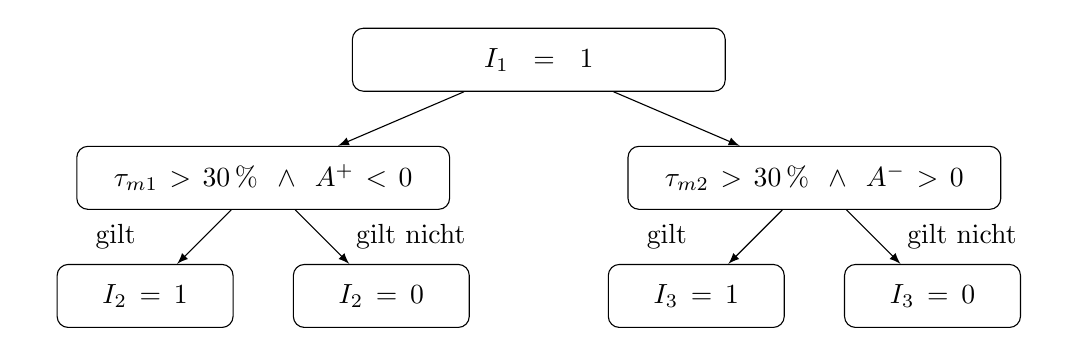
\begin{tikzpicture}[
        grow=down,
        level distance=1.5cm,
        every node/.style={
            draw,
            rounded corners,
            align=center,
            minimum height=0.8cm,
            text width=4.5cm
        },
        edge from parent/.style={draw, -latex},
        level 1/.style={
            sibling distance=7cm
        },
        level 2/.style={
            sibling distance=3cm,
            every node/.style={
                draw,
                rounded corners,
                align=center,
                minimum height=0.8cm,
                text width=2cm
            }
        }
    ]

    \node {$I_1 = 1$}
        child {
            node {$\tau_{m1} > 30\,\% \;\wedge\; A^+ < 0$}
            child {
                node {$I_2 = 1$}
                edge from parent
                node[left, draw=none] {gilt}
            }
            child {
                node {$I_2 = 0$}
                edge from parent
                node[right, draw=none] {gilt nicht}
            }
        }
        child {
            node {$\tau_{m2} > 30\,\% \;\wedge\; A^- > 0$}
            child {
                node {$I_3 = 1$}
                edge from parent
                node[left, draw=none] {gilt}
            }
            child {
                node {$I_3 = 0$}
                edge from parent
                node[right, draw=none] {gilt nicht}
            }
        };

    \end{tikzpicture}
    \caption{Entscheidungsbaum zur Bestimmung der Interventionsmenge $I_j$}
    \label{fig:entscheidungsbaum_interventionsmenge}
\end{figure}


Entsprechend des DTx-Modells würde die Therapieeinheit als Komponente dann verschiedene Interventionen und Gesprächsschritte bündeln, sodass ein unterstützender Prozess entsteht. Die narrative Ebene sorgt für einen nachvollziehbaren Gesprächsverlauf und liefert Motivation, Feedback, Erinnerungen, sowie technische Unterstützung. Die therapeutische Gesprächsinstanz erstellt dann die eigentliche Gesprächsebene des Chatbots.


\section{Gesprächsebene}

Die Gesprächsebene bildet die finale Instanz des entwickelten Frameworks und steuert die sprachliche Synthese der Chatbot-Antwort ($R_t$) zum Zeitpunkt $t$. Diese Ebene unterscheidet sich grundlegend zwischen den beiden experimentellen Bedingungen des Versuchsaufbaus: Während die Kontrollgruppe ($B_K$) eine rein reaktive, auf generischen traumasensiblen Coaching-Regeln basierende Antwort generiert, operiert die Experimentalgruppe ($B_{PSI}$) über eine mathematisch-psychologisch determinierte Verknüpfungslogik.

Für die Experimentalgruppe ($B_{PSI}$) wird das Large Language Model (LLM) mittels des System-Prompts dazu angewiesen, die Antwort nicht ausschließlich semantisch auf den Inhalt der Nutzereingabe ($U_t$) zu beziehen, sondern die zuvor berechneten Steuerungsvariablen exzessiv zu integrieren:
\[
R_t =
\begin{cases}
    \mathcal{G}(U_t,S_t,K_t), & B_K \\[6pt]
    \mathcal{G}(U_t,S_t,Z_t,G_t,I_t,K_t), & B_{PSI}
\end{cases}
\]
Dabei bezeichnet:
\[
\begin{aligned}
R_t &:= \text{generierte Chatbot-Antwort zum Zeitpunkt } t.\\
\mathcal{G} &:= \text{sprachliche Generierungsfunktion des LLM } t,\\
U_t &:= \text{Nutzereingabe zum Zeitpunkt } t,\\
S_t &:= \text{Ergebnis der Sicherheitsprüfung zum Zeitpunkt } t,\\
Z_t &:= \text{PSI-Zustandsanalyse zum Zeitpunkt } t,\\
G_t &:= \text{Unterstützungsziels zum Zeitpunkt } t,\\
I_t &:= \text{Auswahl der Intervention zum Zeitpunkt } t,\\
K_t &:= \text{Kontextanalyse zum Zeitpunkt } t,\\
\end{aligned}
\]
In diesem letzten Schritt wird erneut der Kontext der Interaktion herangezogen und bezüglich des auf EOS-Ebene 5 (\(K_{5t}\)) identifizierte unbewusste Basismotiv (Leistung, Macht, Anschluss oder Freiheit) interpretiert. An dieser Stelle wird geprüft, welche Metaphern, Schlüsselwörter und motivationalen Trigger das LLM wählt, um eine maximale Passung an die Persönlichkeitsstruktur des Nutzers zu erreichen. Die sprachliche Ausgestaltung wird dabei durch das Motivgerüst von $K$ eingefärbt. Ein leistungsmotivierter Nutzer wird über Zielerreichung und Optimierung adressiert, während ein freiheitsmotivierter Nutzer über Autonomie und Selbstbestimmung aktiviert wird. Durch diese strikte Trennung von Inhaltsebene (Nutzeranliegen) und Funktionsebene (PSI-Steuerung) wird sichergestellt, dass der Chatbot nicht lediglich bestehende, dysfunktionale Denkmuster reproduziert, sondern durch gezielte, motivkonforme Impulse zur aktiven Transformation beiträgt.


\section{Basispromt}



\section{Evaluation}
Das primäre Ziel der Evaluation besteht darin, die theoretisch-konzeptionelle Funktionsfähigkeit der modellierten Zustands-, Ziel- und Interventionslogik experimentell zu überprüfen. Es wird explizit keine klinische Wirksamkeitsstudie im therapeutischen Sinne durchgeführt. Vielmehr steht der Nachweis im Vordergrund, ob das Modell unter der Bedingung $B_{PSI}$ in der Lage is, ausgehend von einem initial erfassten Ausgangszustand eine theoriekonforme Intervention auszuwählen, die eine gerichtete, theoretisch fundierte Systemverschiebung auf den psychischen Achsen des Nutzers einleitet \citep{kuhl2005neue}. \\

Für jedes simulierte Interaktionsszenario wird der funktionale PSI-Zustand ($Z$) auf Basis der mathematischen Aggregationslogik zu zwei diskreten Messzeitpunkten evaluiert:
\begin{itemize}
    \item $Z_{t_0}$: Der empirische Ausgangszustand des Nutzers vor der Intervention, abgeleitet aus der relativen Normalisierung der initialen Nutzereingabe ($U_t$).
    \item $Z_{t_1}$: Der tatsächliche, phänomenologische Systemzustand, welcher durch die linguistische Analyse der generierten Chatbot-Antwort ($R_t$) induziert und direkt im Anschluss gemessen wird.
\end{itemize}

Im Rahmen des Systemtests generieren sowohl die Experimentalgruppe ($B_{PSI}$) als auch die Kontrollgruppe ($B_{K}$) auf Basis identischer Szenarien-Inputs eine Antwort $R_t$. Diese Antworten werden anschließend mittels der linguistischen Kriterien aus Tabelle \ref{tab:psi_eos_ebenen_parser} bewertet, um die Ausprägung des tatsächlichen Folgezustands $Z_{t_1}$ mathematisch zu bestimmen und den resultierenden Transformationseffekt im direkten Vorher-Nachher-Vergleich zu analysieren.

\subsection{Metriken und mathematische Operationalisierung}
Um die theoriegeleitete Transformation der funktionalen Systemzustände numerisch zu erfassen, wird kein statischer, numerischer Zielzustand vordefiniert. Die Evaluation fokussiert stattdessen die Überprüfung einer gerichteten Systemverschiebung (\textit{Directional Shift}) auf den theoretisch postulierten Systemachsen. Ein Zustand $Z$ zu einem beliebigen Messzeitpunkt wird über seine relativen Makrosystem-Scores ($\%System$) im vierdimensionalen Raum beschrieben.

Der experimentelle Steuerungseffekt wird direkt über das Differenzenmaß ($\Delta$) der normalisierten Prozentwerte zwischen dem Ausgangszustand ($Z_{t_0}$) und dem tatsächlichen Folgezustand ($Z_{t_1}$) operationalisiert:
\begin{equation}
    \Delta\%System = \%System(Z_{t_1}) - \%System(Z_{t_0})
\end{equation}

\subsubsection{Szenarienspezifische Zielmetriken nach Modulationsannahmen}
Die Erfolgskontrolle basiert auf der gerichteten Veränderung jener psychischen Systeme, die laut den Modulationsannahmen der PSI-Theorie durch die jeweilige Intervention aktiviert werden sollen:
\begin{enumerate}
    \item \textbf{Fokus Erste Modulationsannahme (Willensbahnung):} Das primäre Evaluationsziel bei vorliegender Willenshemmung ist die Aktivierung der Intuitiven Verhaltenssteuerung ($IVS$) zur Auflösung der Blockade des Intentionsgedächtnisses ($IG$). Der Steuerungseffekt ($E_{M1}$) bestimmt sich somit primär über den Zuwachs des IVS-Scores:
    \begin{equation}
        E_{M1} = \Delta\%IVS = \%IVS(Z_{t_1}) - \%IVS(Z_{t_0})
    \end{equation}
    
    \item \textbf{Fokus Zweite Modulationsannahme (Selbstentwicklung):} Das primäre Evaluationsziel bei vorliegender stressinduzierter Hemmung der Selbstentwicklung ist die Wiederherstellung des Selbstzugangs durch Aktivierung des Extensionsgedächtnisses ($EG$) zur Reduktion des fehlerfokussierten Objekterkennungssystems ($OES$). Der Steuerungseffekt ($E_{M2}$) bestimmt sich somit über den Zuwachs des EG-Scores:
    \begin{equation}
        E_{M2} = \Delta\%EG = \%EG(Z_{t_1}) - \%EG(Z_{t_0})
    \end{equation}
\end{enumerate}
Ein positiver Wert ($E > 0$) indiziert den theoriekonformen Systemwechsel, während ein Wert von $E \le 0$ ein Verharren in der dysfunktionalen Blockade oder eine Vertiefung der Problem-Regression signalisiert.

\subsection{Hypothesenformulierung und statistische Auswertung}
Der zentrale statistische Vergleich fokussiert nicht die absolute Qualität einzelner Dialogsequenzen, sondern die relative Überlegenheit der Interventionssteuerung unter der Bedingung $B_{PSI}$ gegenüber der Kontrollbedingung $B_{K}$. Geprüft wird, ob die mathematisch gesteuerte Experimentalgruppe zu einer signifikant stärkere Aktivierung des jeweils indizierten Zielsystems führt. Es werden die folgenden Forschungshypothesen aufgestellt:

\begin{equation}
    H_{1, M1}: E_{M1, B_{PSI}} > E_{M1, B_{K}} \quad \Longrightarrow \quad (\Delta\%IVS)_{B_{PSI}} > (\Delta\%IVS)_{B_{K}}
\end{equation}
\begin{center}
    \begin{minipage}{0.85\textwidth}
    \textit{Die Anwendung des PSI-basierten Modells ($B_{PSI}$) führt bei Szenarien zur ersten Modulationsannahme im Vergleich zu einer konventionellen Kontrollbedingung ($B_{K}$) zu einer signifikant stärkeren Aktivierung der Intuitiven Verhaltenssteuerung ($IVS$).}
    \end{minipage}
\end{center}

\begin{equation}
    H_{1, M2}: E_{M2, B_{PSI}} > E_{M2, B_{K}} \quad \Longrightarrow \quad (\Delta\%EG)_{B_{PSI}} > (\Delta\%EG)_{B_{K}}
\end{equation}
\begin{center}
    \begin{minipage}{0.85\textwidth}
    \textit{Die Anwendung des PSI-basierten Modells ($B_{PSI}$) führt bei Szenarien zur zweiten Modulationsannahme im Vergleich zu einer konventionellen Kontrollbedingung ($B_{K}$) zu einer signifikant stärkeren Aktivierung des Extensionsgedächtnisses ($EG$).}
    \end{minipage}
\end{center}

\vspace{2mm}
Die korrespondierenden Nullhypothesen ($H_0$) lauten dementsprechend:
\begin{align}
    H_{0, M1}: (\Delta\%IVS)_{B_{PSI}} \le (\Delta\%IVS)_{B_{K}} \\
    H_{0, M2}: (\Delta\%EG)_{B_{PSI}} \le (\Delta\%EG)_{B_{K}}
\end{align}
\begin{center}
    \begin{minipage}{0.85\textwidth}
    \textit{Die Anwendung des PSI-basierten Modells ($B_{PSI}$) führt im Vergleich zur Kontrollbedingung ($B_{K}$) zu keiner signifikant stärkeren Aktivierung des jeweils theoriekonformen Zielsystems ($IVS$ bzw. $EG$).}
    \end{minipage}
\end{center}

Da die durch das LLM vergebenen Erkennungs-Scores (Ebenen 1--7) ein ordinales Skalenniveau aufweisen und die berechneten Differenzenmaße ($\Delta\%System$) aufgrund des stochastischen Verhaltens von Sprachmodellen nicht als normalverteilt vorausgesetzt werden können, wird für den nicht-parametrischen Vergleich der verbundenen Stichproben der \textit{Wilcoxon-Vorzeichen-Rang-Test} herangezogen. Das statistische Signifikanzniveau für die Ablehnung der Nullhypothese wird auf einseitig $\alpha = 0{,}05$ festgelegt, bei einer Stichprobenarchitektur von exakt $n = 10$ verbundenen Paaren pro Modulationsannahme.

\subsubsection{Statistische Effektstärke ($r$)}
Ergänzend zur Prüfung des p-Werts wird die standardisierte Effektstärke $r$ berechnet, um die praktische Relevanz der Interventionssteuerung unabhängig vom Signifikanzniveau zu quantifizieren. Da es sich um ein nicht-parametrisches Verfahren handelt, wird $r$ aus der standardisierten Teststatistik $Z_{stat}$ des Wilcoxon-Tests abgeleitet:
\begin{equation}
    r = \frac{|Z_{stat}|}{\sqrt{N}}
\end{equation}
Hierbei entspricht $N = 10$ der Anzahl der Simulationspaare der jeweiligen Bedingungsgruppe. Die Interpretation der Effektstärke erfolgt nach den Schwellenwerten von Cohen: $r \ge 0{,}1$ indiziert einen schwachen, $r \ge 0{,}3$ einen mittleren und $r \ge 0{,}5$ einen starken experimentellen Steuerungseffekt.
